\section{Masinõppe meetodite kvaliteedimõõtude veahinnangud}
\label{section:kvaliteedimõõtude veahinnangud}
Kolm sageli kasutatud kvaliteedimõõtu klassifitseerimismeetodite puhul on õigsus, täpsus ja saagis. Õigsus näitab, kui sagedasti meetod andmepunkte õigesti klassifitseerib (tähistame $\accuracy$). Täpsus mõõdab päris positiivsete klassifikatsioonide sagedust ennustatud positiivsete seast (tähistame $\precision$). Saagis on päris positiivsete klassifikatsioonide sagedus positiivsete andmepunktide seast (tähistame $\recall$).

Tähistagu $i$-ndat andmepunkti elementide paar $(x_i, y_i)$, kus $x_i$ tähistab andmepunkti tunnuseid ning $y_i$ andmepunkti klassi. Antud töös vaatleme ainult binaarse klassifitseerimise ülesannet, kus märgend $y_i$ võib olla üks kahest võimalikust väärtusest, negatiivne klass tähistusega $0$ või positiivne klass tähistusega $1$. Vaatleme meetodi käitumist andmepunktidel, meetodi $A$ puhul andmepunktile vastav klassifikatsioon on $A(x_i) = a_i$. Juhuslikku andmepunkti võime vaadelda juhusliku suurusena $(X, Y)$ ning meetodi klassifikatsiooni selle tunnustel  kui juhuslikku suurust $A$. Selle põhjal defineerime meetodi $A$ kvaliteedimõõdud läbi ooteväärtuste
\begin{align}
    \accuracy &= \mean{A = Y} \enspace, \label{eq:õigsus}\\
    \precision &= \mean{A = Y | A = 1} \enspace, \label{eq:täpsus}\\
    \recall &= \mean{A = Y | Y = 1} \enspace. \label{eq:saagis}
\end{align}

Klassifitseerimismeetodi kvaliteedimõõtude tegelikke väärtusi on praktikas peaaegu võimatu leida. Sageli leitakse neile lähendid rakendades meetodit lõplikul hulgal märgendatud testandmetel.

\subsection{Õigsuse lähend}
Õigsuse, täpsuse ja saagise puhul on nende kõigi analüüs analoogseks. Samas on õigsuse uurimine tehniliselt kõige lihtsam, sest definitsiooni järgi ei sisalda see tinglikku jaotust. Sellel põhjusel uurime õigsust esimesena.
 
Meetodi rakendamise tulemust valimi $i$-ndal andmepunktil tõlgendame kui Bernoulli katset ehk Bernoulli jaotusega juhuslikku suurust $Z_i = [a_i = y_i]$, mille võimalikud väärtused on $1$ ja $0$ vastavalt õige ning vale klassifikatsiooni korral. Meetodi tegelik õigsus $\accuracy$ määrab juhusliku valimi korral iga katse õnnestumise tõenäosuse
\begin{equation*}
    \accuracy = \mean{A = Y} = 0 \cdot \prob{A \neq Y} + 1 \cdot \prob{A = Y} = \prob{a_i = y_i} \enspace.
\end{equation*}

Lähtudes eelnevast saame meetodi õigsust~\eqref{eq:õigsus} lähendada statistilise tõenäosusena üle $N$ andmepunkti suuruse valimi
\begin{equation}
    \label{eq:õigsus lähend}
    \widehat{\accuracy} = \frac{1}{N} \cdot \sum^{N}_{i = 1} Z_i = \frac{1}{N} \cdot \sum^{N}_{i = 1} [a_i = y_i] \enspace.
\end{equation}
Kasutades keskväärtuse, dispersiooni ja Bernoulli jaotuse omadusi avaldame õigsuse lähendi keskväärtuse ning dispersiooni
\begin{align*}
    \mean{\widehat{\accuracy}} &= \frac{1}{N} \cdot \mean{\sum^{N}_{i = 1} Z_i} = \frac{1}{N} \cdot N \cdot \accuracy = \accuracy \enspace, \\
    \variance{\widehat{\accuracy}} &= \frac{1}{N^2} \cdot \variance{\sum^{N}_{i = 1} Z_i} = \frac{1}{N} \cdot \accuracy \cdot (1 - \accuracy) \enspace.
\end{align*}

Kuna suurus $\widehat{\accuracy}$ on ligikaudne väärtus tegelikule õigsusele, tahame märgendada piisavalt suure valimi, et lähendi absoluutne viga $\Delta \accuracy = \widehat{\accuracy} - \accuracy$ oleks üle valimi küllaltki suure tõenäosusega absoluutväärtuselt võimalikult väike.

\subsection{Täpsuse ja saagise lähendid}
Populatsiooni või valimi korral, mille klasside sagedus ei ole tasakaalus, võib õigsus olla eksitav hinnang meetodi kvaliteedi kohta. Valimis mille andmepunktidest 90\% kuuluvad positiivsesse ning 10\% negatiivsesse klassi, kõikide andmepunktide positiivseks klassifitseerimine annab meetodile õigsuse $\accuracy = 0{,}9$. Lisaks hindab õigsus kõiki klassifitseerimisel tehtud vigu ühtemoodi. Kui valepositiivne või valenegatiive klassifikatsioon võib põhjustada palju kahju on oluline tehtud vigu üksteisest eristada.

Täpsus mõõdab päris positiivsete klassifikatsioonide sagedust ennustatud positiivsete seast. Täpsuse hindamiseks läbi statistilise tõenäosuse peame kõigepealt leidma kuidas see avaldub tõenäosuste kaudu
\begin{align}
    \precision &= \mean{A = Y | A = 1} = 0 \cdot \prob{A \neq Y | A = 1} + 1 \cdot \prob{A = Y | A = 1} \nonumber\\
    &= \prob{Y = 1 | A = 1} = \frac{\prob{Y = 1 \land A = 1}}{\prob{A = 1}} \enspace. \label{eq:täpsus tõenäosusesitus}
\end{align}
Tulemuse~\eqref{eq:täpsus tõenäosusesitus} põhjal saame hinnata täpsust~\eqref{eq:täpsus} üle $N$ andmepunkti suuruse valimi
\begin{equation}
    \label{eq:täpsus lähend}
    \widehat{\precision} = \frac{\frac{1}{N} \cdot \sum \limits_{i = 1}^{N} [a_i = 1] \cdot [y_i = 1]}{\frac{1}{N} \cdot \sum \limits_{i = 1}^{N} [a_i = 1]} = \frac{\sum \limits_{i = 1}^{N} [a_i = 1] \cdot [y_i = 1]}{\sum \limits_{i = 1}^{N} [a_i = 1]}\enspace.
\end{equation}

Saagis on päris positiivsete klassifikatsioonide sagedus positiivsete andmepunktide seast. Sarnaselt täpsuse esitusele tõenäosuste kaudu \eqref{eq:täpsus tõenäosusesitus} esitame ka saagise tõenäosuste kaudu
\begin{equation*}
    \recall = \mean{A = Y | Y = 1} = \frac{\prob{Y = 1 \land A = 1}}{\prob{Y = 1}} \enspace,
\end{equation*}
mille põhjal saame saagise \eqref{eq:saagis} lähendi üle valimi arvutada järgnevalt
\begin{equation}
    \label{eq:saagis lähend}
    \widehat{\recall} = \frac{\frac{1}{N} \cdot \sum \limits_{i = 1}^{N} [a_i = 1] \cdot [y_i = 1]}{\frac{1}{N} \cdot \sum \limits_{i = 1}^{N} [y_i = 1]} = \frac{\sum \limits_{i = 1}^{N} [a_i = 1] \cdot [y_i = 1]}{\sum \limits_{i = 1}^{N} [y_i = 1]} \enspace.
\end{equation}

Sellisel kujul lähendite tõenäosuslik hindamine võib olla keeruline, sest nii murru lugejas kui ka nimetajas on ligikaudsed suurused. Lihtsam on uurida lähendit üle valimi tinglikust jaotusest. Antud juhul on tingimuseks kvaliteedimõõdu definitsioonis olev sündmus, näiteks täpsuse puhul $A = 1$. Tinglikule jaotusele vastava valimi leidmiseks kasutame valikumeetodit (\emph{rejection sampling}):
\begin{enumerate}
    \item Võtame jaotusest juhusliku andmepunkti.
    \item Kontrollime andmepunkti vastavust tingimusele.
    \item Kui andmepunkt vastab tingimusele võtame selle valimisse, vastasel juhul mitte.
    \item Kordame kuni on leitud soovitud koguses tingimusele vastavaid andmepunkte.
\end{enumerate}

Valikumeetodi põhjal leiame valimi $A^{+}$, mis koosneb positiivseks klassifitseeritud andmepunktidest, ning valimi $Y^{+}$, mis koosneb positiivse klassiga andmepunktidest. Kasutades vastavaid valimeid avaldame lähendid~\eqref{eq:täpsus lähend} ja~\eqref{eq:saagis lähend} õigsusele~\eqref{eq:eq:õigsus lähend} sarnasel kujul
\begin{align}
    \widehat{\precision} &= \frac{1}{| A^{+} |} \cdot \sum_{i \in A^{+}} [y_i = 1] \enspace, \label{eq:täpsus tinglik lähend}\\
    \widehat{\recall} &= \frac{1}{|Y^{+}|} \cdot \sum_{i \in Y^{+}} [a_i = 1] \label{eq:saagis tinglik lähend}\enspace.
\end{align}
On oluline märgata, et lähendid~\eqref{eq:täpsus tinglik lähend} ja~\eqref{eq:saagis tinglik lähend} on analoogsed õigsuse lähendile~\eqref{eq:õigsus lähend} ning seelle tõttu on nende absoluutsed ja relatiivsed vead samasuguste omadustega.

Lihtsa valikumeetodi puhul on probleemiks tingimuse kontrollimine valimi moodustamisel. Täpsuse puhul on tingimuse kontrollimine lihtne, sest piisab vaid meetodi rakendamisest andmepunktile. Saagise puhul ei pruugi meetod väga hästi toimida, sest tingimuse kontrollimiseks peame välja selgitama andmepunkti tegeliku klassi. Tegeliku klassi leidmine on võrreldes klassifikatsiooni leidmisega kulukas. Valikumeetodi rakendamine saagise lähendamiseks on eriti kulukas, kui positiivse klassiga andmepunktid jaotuses on haruldased. Leidub ülesandeid mille puhul võib positiivse juhtumi esinemissagedus olla $1 \div 10 000$, näiteks tekstist faktide eraldamine. Sellisel juhul peame $1 000$ elemendilise valimi saamiseks märgendama $10$ miljonit andmepunkti. Isesõitvate autode puhul võivad huvipakkuvad sündmused esineda ühel korral miljonist ning seega peaksime naiivse lähenemise korral vaja märgendada ligi miljard andmepunkti. Kuid vajaliku töökindluse saavutamiseks peame selliste sündmustega ikkagi arvestama. See on ka üks põhjus, miks suure töökindlusega praktikas kasutatavate masinõppe algoritmide loomine on keerukas protsess.

\subsection{Õigsuse lähendi absoluutne viga}
Valimi põhjal leitud lähendid kvaliteedimõõtudele sisaldavad viga. Kui tahame veenduda lähendi vastavuses selle täpsele väärtusele tekib küsimus vea suuruse kohta. Vea arvutamiseks peame teadma täpset väärtust, mis ei pruugi olla võimalik. Täpset väärtust teadmata saame viga hinnata tõenäosuslikult. Standardselt seatakse eesmärgiks hinnata kui suur on viga $95\%$ juhtudest.

Üks viis vea tõenäosuslikuks hindamiseks on kasutada konsentratsioonivõrratusi, näiteks Höffdingi võrratust. Höffdingi võrratus on suurte arvude seaduse konkreetne erijuht, mis annab üldistest hinnangutest täpsemaid tõkkeid tõenäosustele. Höffdingi võrratus annab ülemise tõkke tõenäosusele, et tõkestatud paarikaupa sõltumatute juhuslike suuruste summa erineb selle summa keskväärtusest (oodatud väärtusest) vähemalt mingi konstandi võrra~\cite{höffdingi-võrratus,tõenäosusteooria-2-loengukonspekt}. Täpsemalt, kui juhuslikud suurused $Z_1, Z_2, \dots, Z_N$ on sõltumatud ning leiduvad tõkked
\begin{equation*}
    a_i \leq Z_i \leq b_i \enspace, 
\end{equation*}
siis summa $S_N = Z_1 + \dots + Z_N$ ning iga positiivse $c$ korral kehtib
\begin{equation*}
    \prob{| S_N - \mean{S_N} | \geq c} \leq 2 \exp{\left( -\frac{2 c^2}{\sum_{i = 1}^{N}(b_i - a_i)^2}\right)} \enspace.
\end{equation*}

Kuna Bernoulli jaotusega juhuslike suuruste jaoks leiduvad tõkked $0 \leq Z_i \leq 1$ järeldub Höffdingi võrratusest seos
\begin{equation}
    \label{eq:höffding absoluutne viga}
    \prob{\mid \widehat{\accuracy} - \accuracy \mid \geq \frac{c}{N}} \leq 2 \exp{\left( - \frac{2 c^2}{N} \right)} \enspace,
\end{equation}
mille põhjal saame hinnata lähendi $\widehat{\accuracy}$ absoluutse vea alumise tõkke tõenäosust. Kui sätime võrratuse~\eqref{eq:höffding absoluutne viga} parema poole võrdseks olulisusega $\alpha$ avaldub veahinnangu alumine tõke kujul
\begin{equation*}
     \varepsilon := \frac{c}{N} = \sqrt{- \frac{1}{2 N} \cdot \ln{\left( \frac{\alpha}{2} \right)}} \enspace.
\end{equation*}
Tulemuse põhjal saame arvutada valimi vajaliku suuruse
\begin{equation*}
    N \geq - \frac{1}{2 \varepsilon^2} \cdot \ln{\left( \frac{\alpha}{2} \right)} \enspace,
\end{equation*}
et fikseeritud olulisuse korral saavutada soovitud suurusega veahinnang.

\begin{table}[H]
    \centering
    \caption{Valimi suurused kindluse ning absoluutse vea suhtes Höffdinig võrratuse põhjal. Kindluse puhul on sulgudes, mitu normaaljaotuse standardhälvet keskväärtuse ümbruses see katab.}
    \begin{tabular}{l | r r r}
        $1-\alpha$ & $\varepsilon=10\%$ & $\varepsilon=1\%$ & $\varepsilon=0{,}1\%$ \\
    	\hline
    	$99\% \enspace (3\sigma)$ & $265$ & $26492$ & $2649159$ \\
    	$95\% \enspace (2\sigma)$ & $185$ & $18445$ & $1844440$ \\
    	$68\% \enspace (1\sigma)$ & $92$  & $9163$  & $916291$  \\
    \end{tabular}
    \label{tab:höffding absoluutne viga}
\end{table}

\begin{figure}[H]
    \begin{center}
        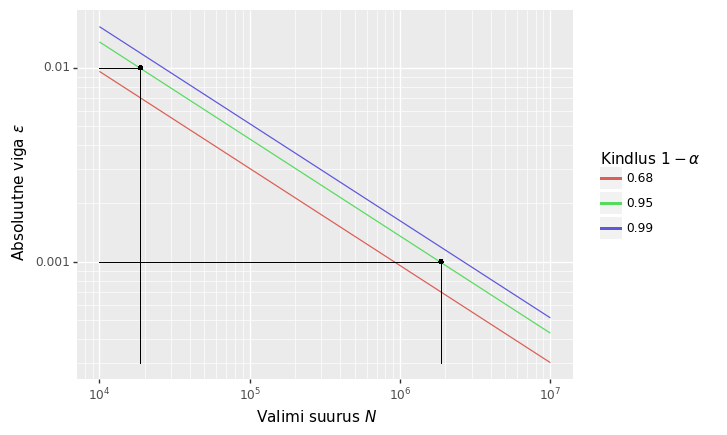
\includegraphics[width=\textwidth]{hoeffding_absoluutne_viga}
    \end{center}
    \caption{Valimi suurused olulisuse ning absoluutse vea suhtes Höffdinig võrratuse põhjal kindlusega $1-\alpha$.}
    \label{fig:höffding absoluutne viga}
\end{figure}

Tabelis~\ref{tab:höffding absoluutne viga} on vajalik valimi suurus soovitud kindluse ja lähendi absoluutse vea suhtes Höffdingi võrratuse põhjal, kindluse puhul on sulgudes, kui mitu normaaljaotuse standardhälvet $\sigma$ keskväärtuse ümbruses see katab. Näiteks kui tahame olla $95\%$ kindlad, et valimi põhjal arvutatud õigsus $\widehat{\accuracy}$ erineb algoritmi tegelikust õigsusest kuni ühe protsendi võrra, peame õigsust hindama valimil suurusega vähemalt $18445$. Joonisel~\ref{fig:höffding absoluutne viga} on sama mõttekäik visuaalselt.

Õigsuse lähendi absoluutse vea hindamiseks saame ka kasutada asjaolu, et suurused $Z_i$ on Bernoulli jaotusega. See tähendab, et summa
\begin{equation*}
    S_N = \sum^{N}_{i = 1} Z_i \enspace,
\end{equation*}
on binoomjaotusega. Mingi binoomjaotusega juhusliku suuruse $X$ puhul tähistatakse seda $X \sim \mathcal{B}(n, p)$, kus parameeter $n$ on Bernoulli katsete arv ja $p$ katse õnnestumise tõenäosus. Sellest lähtudes väidame järgnevat
\begin{equation*}
    S_N \sim \mathcal{B}(N, \accuracy) \enspace.
\end{equation*}
Seega on õigsuse lähend $\widehat{\accuracy}$ skaleeritud binoomjaotusega juhuslik suurus. Eespool leitud Höffdingi võrratusel põhinevad tõkked selle omadusega ei arvestanud ning olid binoomjaotuse parameetrist $p$ sõltumatud, tegu oli konservatiivse hinnanguga. Höffidngi võrratus on universaalne üle kõikide binoomjaotuse parameetrite $p$, millest halvim variant realiseerub juhul $p = 0{,}5$. Binoomjaotusel põhinevad tõkked on täpsed ning annavad aimu Höffidngi võrratuse tulemuste ebatäpsustest. Lisaks näitavad binoomjaotusel põhinevad arvutused kuidas meetodi tegelik õigsus $\accuracy$ mõjutab tulemusi.

Kasutades teadmist, et uuritav summa on binoomjaotusega leiame jaotuse parameetritest sõltuva hinnangu. Olulisuse $\alpha$ korral leiame absoluutse veahinnangu tõkke $\varepsilon$ lähtudes võrrandist
\begin{equation}
    \label{eq:binoomjaotus absoluutne viga}
    \prob{\mid \widehat{\accuracy} - \accuracy \mid \geq \varepsilon} = \alpha \enspace,
\end{equation}
valime protsendipunktid, arvud millest $S_N$ võtab väiksemaid väärtusi protsendipunktile vastava tõenäosusega, sümmeetriliselt
\begin{align*}
    \prob{\widehat{\accuracy} \leq \accuracy - \varepsilon} &= \frac{\alpha}{2} \enspace,\\
    \prob{\widehat{\accuracy} <    \accuracy + \varepsilon} &= 1 - \frac{\alpha}{2} \enspace,
\end{align*}
kui eraldame binoomjaotusega juhusliku suuruse $S_N$ ühele poole võrratuse märki jõuame tulemuseni
\begin{align*}
    \prob{S_N \leq N \cdot (\accuracy - \varepsilon)} &= \frac{\alpha}{2} \enspace,\\
    \prob{S_N < N \cdot (\accuracy + \varepsilon)} &= 1 - \frac{\alpha}{2} \enspace.
\end{align*}
Paremale poole võrratuse märki tekkinud avaldised on $S_N$ jaotuse vastavalt $\frac{\alpha}{2}$ ja $1-\frac{\alpha}{2}$ protsendipunktid, 
\begin{align*}
    q_1 &= N \cdot(\accuracy-\varepsilon) \enspace, \\
    q_2 &= N \cdot(\accuracy+\varepsilon) \enspace. \\
\end{align*}
Fikseeritud olulisuse ja binoomjaotuse parameetrite korral võime protsendipunktid arvutada kasutades $S_N$ jaotuse omadusi. 

Absoluutse vea tõkkeks $\varepsilon$ võrrandist~\eqref{eq:binoomjaotus absoluutne viga} valime suurema protsentipunktide põhjal arvutatud veahinnangutest
\begin{equation}
    \label{eq:binoomjaotus absoluutne viga tõke}
    \varepsilon = \max \left( \accuracy - \frac{q_1}{N} , \frac{q_2}{N} - \accuracy \right) \enspace.
\end{equation}
Parameetri $N$ kasvades koondub binoomjaotus normaaljaotuseks~\cite{tõenäosusteooria-algkursus}. Seega suuremate $N$ väärtuste puhul on binoomjaotus sümmeetriline, järelikult erinevad $q_1$ ja $q_2$ põhjal arvutatud veahinnangute väärtused tegelikkuses vähe. Tulemust \eqref{eq:binoomjaotus absoluutne viga tõke} kasutades saame arvutada vajaliku valim suuruse soovitud olulisuse suhtes, kuid selle jaoks peame oletama mudeli tegelikku õigsust $\accuracy$.

\begin{table}[H]
    \centering
    \caption{Valimi suurused absoluutse vea ning oletatava õigsuse suhtes binoomjaotuse põhjal kindlusega $95\%$. Sulgudes on kirjas kui mitu korda on Höffdingi võrratusel põhinev valim suurem.}
    \begin{tabular}{l | r r r}
        $\accuracy$ & $\varepsilon = 10\%$ & $\varepsilon = 1\%$ & $\varepsilon = 0,1\%$ \\
    	\hline
    	$70\%$ & $75\enspace(2{,}47)$ & $8100\enspace(2{,}28)$ & $806289\enspace(2{,}29)$ \\
    	$90\%$ & $35\enspace(5{,}29)$ & $3600\enspace(5{,}12)$ & $347020\enspace(5{,}32)$ \\
    	$95\%$ & $20\enspace(9)$      & $1850\enspace(9{,}97)$ & $183285\enspace(10{,}06)$ \\
    \end{tabular}
    \label{tab:binoomjaotus absoluutne viga}
\end{table}

\begin{figure}[H]
    \begin{center}
        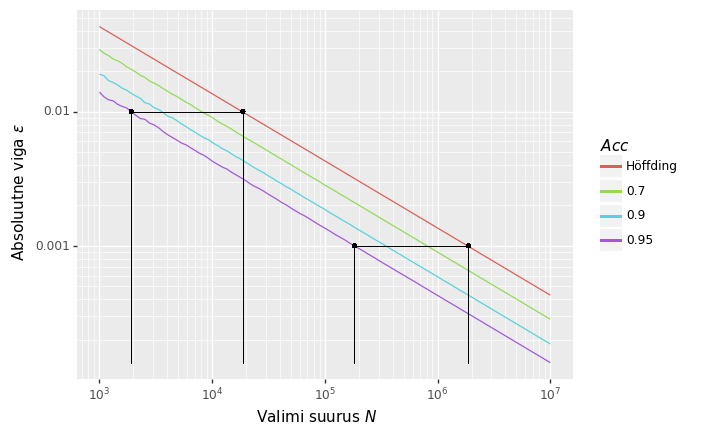
\includegraphics[width=\textwidth]{binoomjaotus_absoluutne_viga}
    \end{center}
    \caption{Valimi suurused absoluutse vea ning oletatava õigsuse suhtes binoomjaotuse põhjal kindlusega $95\%$.}
    \label{fig:binoomjaotus absoluutne viga}
\end{figure}

Tabelis~\ref{tab:binoomjaotus absoluutne viga}ja joonisel~\ref{fig:binoomjaotus absoluutne viga} on valimi vajalikud suurused meetodi oletatud õigsuse ja absoluutse veahinnangu soovitud suuruse suhtes binoomjaotuse omaduste põhjal kindlusega $95\%$. Võrdluseks on olemas ka Höffdingi võrratusel põhinevad tulemused sama kindlusega, joonisel eraldi joonena, tabelis on sulgudes kirjas kui mitu korda on Höffdingi võrratuse põhine valim suurem. Eeldusel, et algoritmi tegelik õigsus on $90\%$, absoluutse vea kuni üks protsent jaoks vajame valimit suurusega vähemalt $3600$, mis on umbes viis korda väiksem kui valim, mida vajasime Höffdingi võrratuse põhjal.

\subsection{Õigsuse lähendi relatiivne viga}
Lisaks ligikaudse väärtuse absoluutsele veale kasutatakse lähendi headuse mõõtmiseks relatiivset viga. Õigsuse lähendi relatiivse vea keskväärtus ja dispersioon avalduvad järgnevalt
\begin{align*}
    \mean{\frac{\widehat{\accuracy}}{\accuracy} - 1} &= \frac{1}{\accuracy} \cdot \mean{\widehat{\accuracy}} - 1 = 1 - 1 = 0 \nonumber \enspace, \\
    \variance{\frac{\widehat{\accuracy}}{\accuracy} - 1} &= \frac{1}{\accuracy^2} \cdot \frac{\accuracy \cdot (1 - \accuracy)}{N} = \frac{1}{N} \cdot \frac{1 - \accuracy}{\accuracy} \enspace.
\end{align*}
Kui avaldame lähendi relatiivse ja absoluutse vea hajuvuse suhte, leiame et kõrge õigsuse korral on õigsuse lähendi veahinnangud ligikaudu sama hajuvusega
\begin{equation*}
    \variance{\frac{\widehat{\accuracy}}{\accuracy}} \div \variance{\widehat{\accuracy} - \accuracy} =
    \left( \frac{1}{N} \cdot \frac{1 - \accuracy}{\accuracy} \right) \div \left( \frac{1}{N} \cdot \accuracy \cdot (1 - \accuracy) \right) = \frac{1}{\accuracy^2} \enspace.
\end{equation*}

Nagu absoluutse veahinnangu puhul on meie eesmärk ka relatiivse veahinnangu puhul seda absoluutväärtuselt minimeerida. Seega võime küsida kui suurt valimit vajame, et relatiivne viga oleks piisavalt suure kindlusega võimalikult väike.

Õigsuse lähend sisaldab binoomjaotusega juhuslikku suurust. Järelikult saame ka relatiivset viga tõenäosuslikult hinnata kasutades binoomjaotuse omadusi. Lähtudes võrrandist
\begin{equation}
    \label{eq:binoomjaotus relatiivne viga}
    \prob{\left| \frac{\widehat{\accuracy}}{\accuracy} - 1 \right| \geq \varepsilon} = \alpha \enspace,
\end{equation}
millest eraldame tõenäosusmärgi aluses võrratuses binoomjaotusega juhusliku suuruse $S_N$ ühele poole võrratusemärki
\begin{align*}
    \prob{S_N \leq N \cdot \accuracy \cdot (1-\varepsilon)} &= \frac{\alpha}{2} \enspace, \\
    \prob{S_N <    N \cdot \accuracy \cdot (1+\varepsilon)} &= 1 - \frac{\alpha}{2} \enspace,
\end{align*}
oleme avaldanud olulisusele vastavad protsendipunktid
\begin{align*}
    q_1 &= N \cdot \accuracy \cdot (1-\varepsilon) \enspace, \\
    q_2 &= N \cdot \accuracy \cdot (1+\varepsilon) \enspace.
\end{align*}

Relatiivse vea tõkkeks $\varepsilon$ võrrandist~\eqref{eq:binoomjaotus relatiivne viga} valime suurema protsendipunktide põhjal avalduva veahinnangu
\begin{equation*}
    \varepsilon = \max \left( 1 - \frac{q_1}{N\cdot\accuracy} , \frac{q_2}{N\cdot\accuracy} - 1 \right) \enspace.
\end{equation*}
Tulemuse põhjal saame leida valimi vajalikud suurused olulisuse suhtes.

\begin{table}[H]
    \centering
    \caption{Valimi suurused relatiivse vea ning eeldatud õigsuse suhtes binoomjaotuse põhjal kindlusega $95\%$.}
    \begin{tabular}{l | r r r }
        $\accuracy$ & $\varepsilon=10\%$ & $\varepsilon=1\%$ & $\varepsilon=0{,}1\%$ \\
    	\hline
    	$70\%$ & $161$ & $16331$ & $1646727$ \\
    	$90\%$ & $53$  & $4176$  & $425856$  \\
    	$95\%$ & $20$   & $1926$  & $202223$  \\
    \end{tabular}
    \label{tab:binoomjaotus relatiivne viga}
\end{table}

\begin{figure}[H]
    \begin{center}
        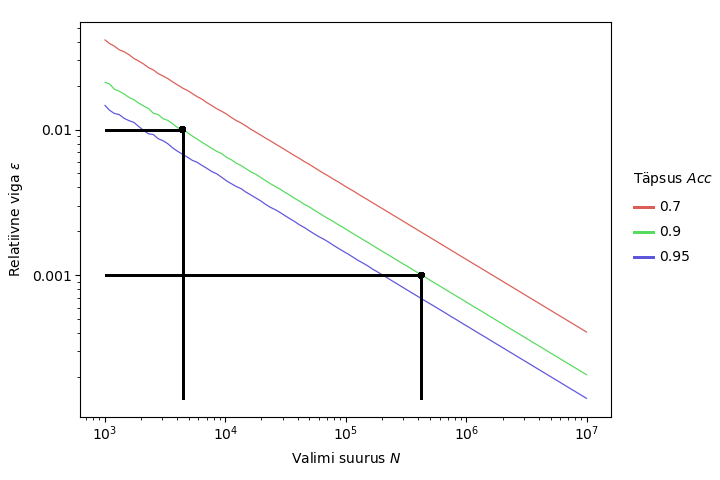
\includegraphics[width=\textwidth]{binoomjaotus_relatiivne_viga}
    \end{center}
    \caption{Valimi suurused relatiivse vea ning eeldatud õigsuse suhtes binoomjaotuse põhjal kindlusega $95\%$.}
    \label{fig:binoomjaotus relatiivne viga}
\end{figure}

Tabelis~\ref{tab:binoomjaotus relatiivne viga} ja joonisel~\ref{fig:binoomjaotus relatiivne viga} on valimi vajalikud suurused meetodi oletatud õigsuse ja relatiivse veahinnangu soovitud suuruse suhtes binoomjaotuse omaduste põhjal kindlusega $95\%$.

\subsection{Tulemuste empiiriline testimine}
Teoreetilisi tulemusi on alati hea praktiliselt kontrollida. Nii saame leide lihtsasti valideerida ning lihtsasti avastada paljud  arvutusvead.

\begin{figure}[H]
    \begin{center}
        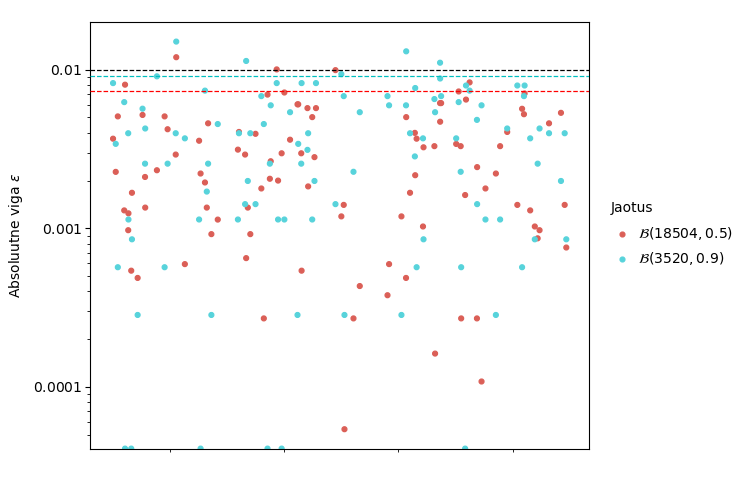
\includegraphics[width=\textwidth]{absoluutne_viga_statistiline_test} 
    \end{center}
    \caption{Höffdingi võrratusel (punane) ja binoomjaotusel (sinine) põhinevate veahinnangute empiiriline test lähendi veaga kuni $1\%$ saamiseks kindlusega $95\%$. Binoomjaotusega summad $S_N$ õigsuse hinnangutes on juhuslikult genereeritud vastavatest jaotustest, punktid joonisel tähistavad summale vastava õigsuse hinnangu absoluutse vea absoluutväärtust. Värvilised jooned märgivad empiiriliselt saadud $0{,}95$ protsendipunkte, must joon nende oodatud asukohta.}
    \label{fig:höffding ja binoomjaotus absoluutne viga empiiriline test}
\end{figure}

Näiteks Höffdingi võrratuse põhjal kindlusega $95\%$ kuni ühe protsendise absoluutse veahinnanguga õigsuse lähendi saavutamiseks vajame valimit suurusega vähemalt $18445$. Oletades, et klassifitseerimismeetodi tegelik õigsus on $90\%$ vajame binoomjaotuse hinnangu põhjal selleks vähemalt $3600$ andmepunkti. Joonisel~\ref{fig:höffding ja binoomjaotus absoluutne viga empiiriline test} on antud näite empiiriline test, kus summa
\begin{equation*}
    S_N = \sum_{i = 1}^N Z_i \enspace,
\end{equation*}
on juhuslikult genereeritud jaotusest $\mathcal{B}(18445; 0{,}5)$ Höffdingi võrratuse puhul (punane) ning $\mathcal{B}(3600; 0{,}9)$ binoomjaotuse hinnangu puhul (sinine). Punktid joonisel tähistavad genereeritud summal põhineva lähendi absoluutset viga
\begin{equation*}
    \varepsilon = \left| \frac{S_N}{N} - p \right| = \left| \widehat{\accuracy} - \accuracy \right| \enspace,
\end{equation*}
ning must joon veahinnangu absoluutväärtuse ülemist tõket, millest veahinnang $\varepsilon$ peaks olema väiksem $95\%$ juhtudest. Punane ja sinine joon on vastava jaotuse puhul tõmmatud läbi empiirilise testimise tulemusel saadud punkti, millest $95\%$ jäävad allapoole. Binoomjaotuse hinnang on täpne ning langes ka antud juhul oodatule lähedale. See-eest langes punane joon oodatust allapoole. Kuna Höffdingi võrratus ülehindab valimi valjalikku suurust on punase joone langemine tema oodatud asukohast allapoole loomulik, sest suurem valim tähendab täpsemat lähendit ja seega väiksemat viga.